\documentclass[journal]{IEEEtran}
% *** CITATION PACKAGES ***
\usepackage{url}
\usepackage{cite}
\usepackage{graphicx}
\usepackage{amsmath}
\interdisplaylinepenalty=2500
\usepackage{array}
\usepackage{multirow}
\usepackage{lipsum}% http://ctan.org/pkg/lipsum
\ifCLASSOPTIONcompsoc
\usepackage[caption=false,font=normalsize,labelfont=sf,textfont=sf]{subfig}
\else
\usepackage[caption=false,font=footnotesize]{subfig}
\fi
\ifCLASSOPTIONcaptionsoff
\usepackage[nomarkers]{endfloat}
\let\MYoriglatexcaption\caption
\renewcommand{\caption}[2][\relax]{\MYoriglatexcaption[#2]{#2}}
% lipsum allows figs/tables to cross-double rows. 
\fi


\begin{document}
	% Do not put math or special symbols in the title.
	\title{Neutron Spectrum Characterization}
	
	\author{Nicholas~Quartemont}
	
	% The paper headers
	\markboth{Neutron Spectrum Characterization}%
	% A title should better capture what the article is about to draw readers in.  This to me sounds like a review article, which this is not
	{Shell \MakeLowercase{\textit{et al.}}: Neutron Spectrum Characterization }

	% make the title area
	\maketitle
	
	% This first commit show a technique that makes it easier to edit and see the edits.  If each sentence is it's own line, then the diff between the files will only show lines that changed.  Otherwise, you have to find the change, which may be small, in a para of text.
	\begin{abstract}
		\ This paper outlines a foil activation experiment performed at the Air Force Institute of Technology neutron pile.
The purpose of the experiment was to measure the neutron flux spectrum in stringer 2 using foil activation unfolding techniques such as STAYSL. 
Due to facility limitations, the unfolding analysis was conducted on an experiment with a test snout performed at the National Ignition Facility (NIF). 
Foil activation experiments are an indirect method of measuring an incident neutron flux and are preferred in high flux environments that will damage electronics or for size constraints. 
Foil activities produced from threshold and non-threshold reactions were analyzed using a high purity germanium detector that resulted in time-corrected activities post-irradiation in the range of 100 Bq to 10 kBq. 
The NIF experiment utilized aluminum, gold, indium, and zirconium foils of varying mass at the pinhole, basket, and kinematic base locations of the snout. 
The irradiation planned for the neutron pile also included tungsten and manganese. 
The incident neutron fluence was unfolded from the activities and nuclear data with a MCNP simulated NIF initial spectrum and a flat spectrum. 
The results for the pinhole and basket show varying physical results, while both have p-values under 0.01. 
However, the results for the basket do not match intuition
% or simulation?
and likey requires a better starting spectrum. 
The result for the kinematic base shows a similar result to the pinhole. 
However, the p-value is near 0.9, which indicates the result is not likely to be representative of the activities produced. 
% I thought you were shooting for 0.95 and above?
The kinematic base is a significant change from the initial source spectrum and requires a better simulated starting spectrum. 
	\end{abstract}
	
	% Note that keywords are not normally used for peerreview papers.
	\begin{IEEEkeywords}
		neutron flux unfolding, foil activation, high purity germanium, STAYSL 
	\end{IEEEkeywords}
	
	\IEEEpeerreviewmaketitle
	
	\section{Introduction}
	\IEEEPARstart{C}{haracterizing} the energy dependent neutron environment has many applications to the nuclear sciences community. 
Determining a neutron flux is important for experiments where the neutron flux requires validation or is not well modeled. 
Neutrons can be detected using a variety of methods, such as Bonner spheres, long counters, He-3 based detectors, or proton recoil scintillators \cite{Knoll}. 
% From a spectroscopy persepective, TOF must be mentioned.
Foil activation experiments can also be performed to acquire an indirect measurement of the incident neutron fluence on a set of activation foils. 
Activation experiments are essential for testing that requires small geometry to fit in the apparatus or in situations where electronics equipment for higher fidelity measuring techniques will be damaged. 
	
	\ This work aims to characterize the neutron spectrum in the Air Force Institute of Technology's (AFIT) Building 470 neutron pile constructed in the 1960s, which contains a plutonium-beryllium (PuBe) neutron source \cite{NETF}. 
Previous studies have accomplished results indicating changes to the neutron source term and modeled the neutron flux at various positions \cite{Bevins,Will}. 
However, the source characterization is still not entirely known. 
	
% write in the past tense, since that is when everything occured
	\ The neutron source characterization was performed with a foil activation experiment. 
The foils were analyzed using a calibrated high purity germanium (HPGe) detector to determine time corrected activities post-irradiation. 
The HPGe was calibrated for energy and efficiency to back out the initial foil activities post-irradiation. 
	
	\ The pile activation results are not used in the final neutron flux analysis due to issues with the HPGe at AFIT. 
Instead, this work analyzed an experimental setup at the National Ignition Facility (NIF). 
The NIF foil activation experiment was performed on a snout for a shot performed in March 2018\cite{Bogetic}. 
The goal of the NIF experiment was to characterize the NIF source in the aluminum snout which has applications for exploring cross-section uncertainties if there are unexpected results. 
The incident neutron flux was determined from the foil activation results using Pacific Northwest National Laboratory (PNNL) STAYSL %cite?
, which uses generalized least-square minimization to determine the flux spectrum for given foil activities and nuclear data.

% Generally, you want to close the first section with a couple of sentences describing the layout of the paper.

	\section{Problem Description}
% Most of this section is background or theory, not a problem description. Most can be combined with section III.
	
% This introduction paragraph needs work.  Use it to introduce the problem, describe the sub sections to follow, and point to further information.
    \ The neutron spectrum characterization requires information from the foil activities. 
The theory and problem statement contributing the foil activation involves the neutron flux environment, foil activation, HPGe spectroscopy, and neutron flux unfolding. 
Supporting documentation and work performed is available on Github\cite{Me}. 
	
	\subsection{Building 470 Pile Neutron Environment }
	\ The neutron pile was modeled in MCNP version 6.1 %need to always cite the first mention of a code
based on previous work to gauge expected activation rates and to determine saturation activities\cite{Will}. 
The setup of foil placement and PuBe source is shown in Figure \ref{fig:pile}. 
The pile has stringers with fabricated placements for the source and foils to help ensure repeatability of measurements. 
	
	\begin{figure}[h!]
		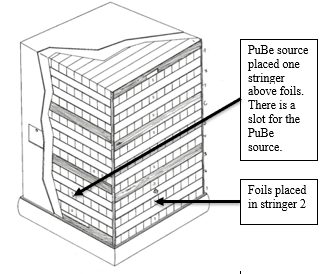
\includegraphics[width=\linewidth]{Figures/PileSetup.png}
		\caption{Activation foil setup for Building 470 graphite pile irradiation.}
		\label{fig:pile}
	\end{figure}
% In the figure, I would simplify the top callout to say "PuBe source placed in designated slot one stringer above the foils."

	\ The starting PuBe neutron spectrum, shown in Figure \ref{fig:PuBE}, ends at 11 MeV and peaks near 3.5 MeV. 
However, there is significant thermalization of the starting PuBe spectrum by the graphite pile as shown in the simulated stringer 2 spectrum in Figure \ref{fig:Spec1}. 
The simulated spectrum was used to select activation foils based on the modeled foil activation rates, discussed in Section ???. 
	
	\begin{figure}[h!]
	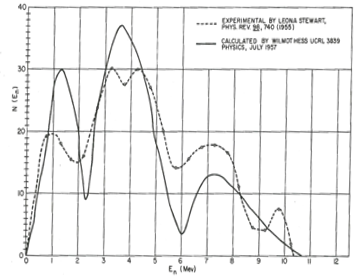
\includegraphics[width=\linewidth]{Figures/PuBe.png}
	\caption{PuBe neutron emission source spectrum.}
	\label{fig:PuBE}

	\vskip 0.25cm

	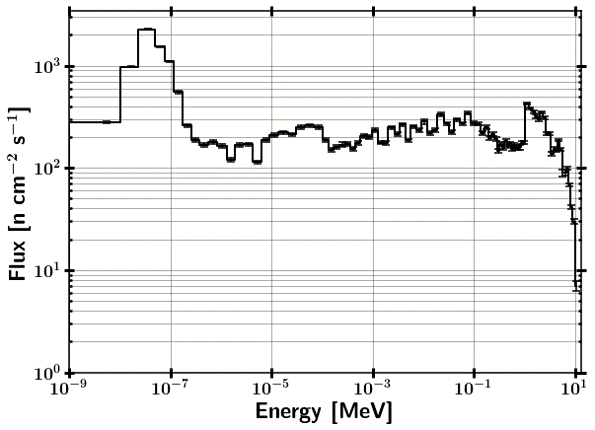
\includegraphics[width=\linewidth]{Figures/PileSpec.png}
	\caption{Foil activation neutron flux spectrum (all statistical errors are under 1.5 percent).}
	\label{fig:Spec1}
	\end{figure}
	% having the same axis would be useful to compare figs 2 and 3

	
	\subsection{NIF Snout Experiment}
	
	\ A passive foil activation experiment was performed in 2018 at the NIF. 
A snout composed of aluminum was mounted to the Target and Diagnostic Manipulator (TANDM) 90-348. 
Three foil activation diagnostic packs of aluminum, zirconium, indium, and gold were placed in the nose cap pinhole (7 cm from source), filter basket (41 cm), and kinematic base (110 cm). 
The aluminum foil was not used in the pinhole. 
Figure \ref{fig:NIF} displays the snout with the activation foil sites \cite{Bogetic}. 
	
	\begin{figure}[h!]
		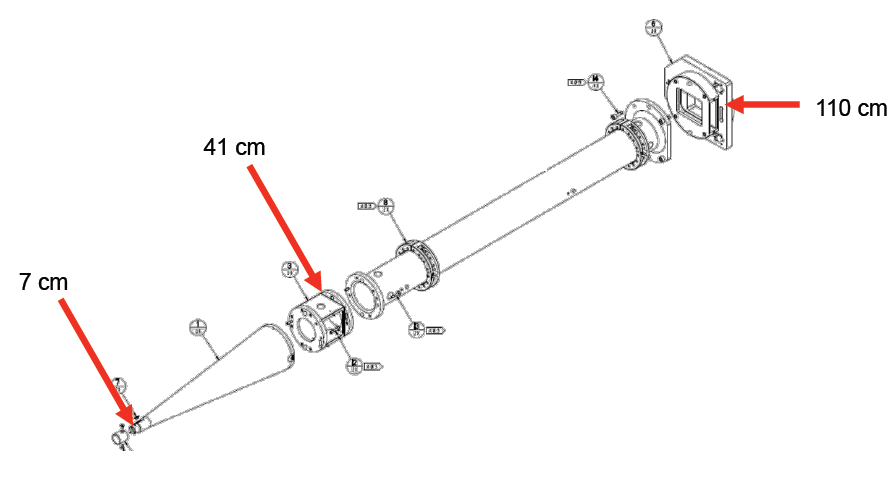
\includegraphics[width=\linewidth]{Figures/NIF.png}
		\caption{Passive NIF snout foil activation locations.  Foils were placed in the nose cap pinhole (7 cm from source), filter basket (41 cm), and kinematic base (110 cm).}
		\label{fig:NIF}
	\end{figure}
%I'd remove the text callout in the figure	
	
	\ The NIF source is a deuterium-tritium (DT) capsule which have neutrons at a nominal energy of 14 MeV. 
The spectrum of neutrons used as a source term %for what? a simulation? More description of this is needed
is shown in Figure \ref{fig:NIFSRC}. 
	
	\begin{figure}[h!]
		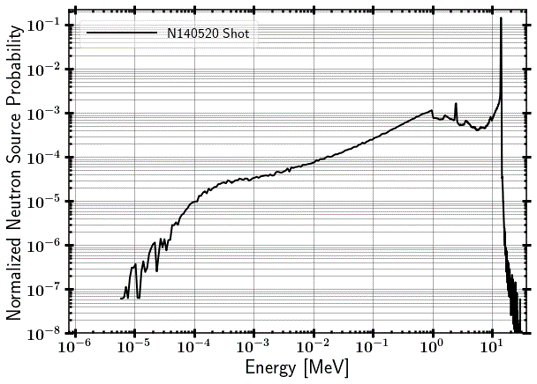
\includegraphics[width=\linewidth]{Figures/NIFSRC.png}
		\caption{A typical NIF D-T neutron source spectrum for high-yield indirect drive shots.}
		\label{fig:NIFSRC}
	\end{figure}
	
	\subsection{Foil Activaiton}
% This section feelsmore relevant to a lab report or thesis.  For a journal article, you can reference sources for foil constraints and highlight whichever affected you selection process.  You can then show the equuations you used to get the time zero activities, and the corrections applied, from the counts.  For example, you didn't explicitly do a backgroud count to subtract, this was done via fitting, so the equation and description don't match what was done and is more academic in nature.

Foil activation can be used with published 	nuclear data to provide an estimate of the incident flux on the foils by unfolding techniques. 
The production rate of radioactive isotopes is negated by radioactive decay processes, which place an upper limit on the radioactivity of a foil \cite{Knoll}. 
The saturated activity, ($A_{\infty}$), for a given reaction is given by: 

% Some of the rest of the article reflects a different thechnique that can also be used, and I left as is when each partial line had its own line number.  This will also directly show the edits made.
	\begin{equation} \label{eq:InfReactionRate}
	A_{\infty} = R = \int_{E1}^{E2} \phi(E) \Sigma(E)_{act} V_{foil} 
	\:dE 
	\end{equation}
	
\noindent the saturated activity is equivalent to the reaction rate (R), which is a function of the energy dependent flux ($\phi$), the macroscopic reaction cross-section for the activation reaction channel($\Sigma(E)_{act}$), and the volume of the foil ($V_{foil}$). 
The energy term ($E1$) is zero in many cases; however, threshold reactions require the incident neutron to be of higher energy to enable the reaction channel. 
	
	A correction needs to be made in cases where the activation is not sufficient 
	to fully saturate the foil. At six half-lives a foil will have reached 
	approximately 98\% of its saturation activity, neglecting spatial and energy 
	self-shielding effects \cite{Knoll}. The activation of the foil for a given 
	irradiation time ($t_{i})$ is given as a function of the decay 
	constant: 

% Some of the subscripts are a bit long, which makes the equations a bit unweildy.  Feel free to modify to something else
	\begin{equation} \label{eq:ReactionRate}
	A_{0} = A_{\infty}(1-e^{-\lambda t_{i}}) 
	\end{equation}
	
	Experimental measurements also can be corrected to deduce the original activity 
	of the foil, immediately after irradiation. The measured counts, $C$, is reduced 
	by the background counts, $B$. A corrects for the 
	radioactive decay for the time between the end of 
	irradiation and the start of counting ($t_{decay}$). A similar correction factor based on 
	the count time, $t_{count}$ provides a correction for radioactive decay during counting. 
	Additionally, the detector efficiency for the given gamma-ray energy, $\epsilon$,  
	and relative gamma intensity, $I_{\gamma}$, must be taken into account. The 
	gamma intensity may also include a branching ratio if applicable to the decay 
	mechanism. All corrections included, less self-shielding effects, provide a 
	formulation for converting counts to post-irradiation activity as: 
	
	\begin{equation} \label{eq:MeasActivity}
	A_{0} = \frac{\lambda (C-B) e^{\lambda t_{decay}}}{\epsilon (1-e^{-\lambda 
			t_{count}})I_{\gamma}}
	\end{equation}
	
	The formula can be simplified in the limit of irradiation times much less that 
	the half-life of the activation products. In this case, the reaction rate is 
	much larger than the decay from radiation, so the rate of production of the 
	radioisotope is driven only by the reaction rate. The time integrated flux, 
	or neutron fluence ($\Phi$), can be used to determine the total reactions, $R_{total}$,
	over an irradiation period, given by:
	
	\begin{equation} \label{eq:NIFrxnRate}
	R_{total} = \int_{E1}^{E2} \Phi(E) \Sigma(E) _{act} V_{foil} 
	\:dE 
	\end{equation}
% Is Eq 4 used anywhere?
	
	\ The foils selected must meet several requirements for this experiment. 
A list of the various requirements that are of importance for a neutron activation foil experiment with energies in the range of thermal to approximately 11 MeV are summarized below \cite{Knoll,Luciano2012a,Kuijpers1977}.
	
	\ The reaction neutron cross-section is extremely important for foil 
	activation, and there are a few key parameters that should be considered. 
	First, the magnitude of the cross-section determines the 
	reaction rate of the product nuclides. A large cross-section allows for 
	more activation, and therefore better results when analyzing the activation 
	foils. Second, the uniqueness of the cross-section shape is used to unfold 
	the incident neutron energy spectrum. An (n,$\gamma$) cross-section may 
	peak in a particular region, which is essential to providing information of the 
	neutron flux in that energy region. Alternatively, a threshold reaction, 
	such as an (n,2n), is important for providing information of the flux at 
	higher energies. Third, the selected foils for an experiment should cover  
	the entire energy range of the incident neutron flux. Finally, the cross-section
	must be well characterized with low uncertainty over the neutron energy range of 
	interest.
	
	\ The decay constant of the product nuclides is important. The 
	half-lives applicable for a particular experiment depend on the time 
	post-irradiation that the foils can be counted. A long lived radioisotope 
	will be available for counting for longer times, but the activity will be 
	reduced due to the lower decay constant. The opposite is true for short 
	half-lives. A half-life on the order of an hour to a few years is in the 
	right direction; however, the half-life must also be balanced with the 
	production of the radioisotope to understand the entire picture. 
	
	\ The elemental and chemical purity of the activation foil should be 
	well known. An unknown composition foil will likely cause erroneous 
	results. 
	
	\ Interfering reaction channels and decay emissions should be avoided. 
	An example of this is natural copper, which has multiple 511 keV emissions 
	from different reaction channels. It is difficult to distinguish these 
	gamma-rays to determine activation in counting. Similar problems arise in 
	multi-isotope materials that have multiple reactions producing the same 
	nuclide. For example, a Cadmium-106 (n,$\gamma$) reaction produces the same 
	isotope as a Cadmium-108 (n,2n) reaction. 
	
	\ The activation foil should be optically this so as to not cause 
	perturbations of the neutron flux. An additional benefit of relatively thin 
	foils is that the gamma-ray emissions are not significantly attenuated 
	through self-shielding. The neutron flux should ideally also not be 
	changing substantially over the foil region. In general adding additional foils helps to improve the unfolding results, as long as the entire foil set remains optically thin  \cite{Vagena2018b}. 
	
	\ The decay nature of the product nuclide should be a gamma-ray 
	emitter. 
	% Beta spectroscopy is available as well and something that should be considered for NIF
	Gamma-ray detection can provide fine energy resolution to 
	determine activation due to specific reaction channels. The discrete gamma-ray emissions provide a means of 
	determining the source and magnitude of the the foil activation. The energy 
	of the gamma is also of importance. Semiconductor detection methods have a 
	peak intrinsic efficiency near 100 keV with some variance depending on if 
	it p-type or n-type. 
	
	\subsection{HPGe Calibration}
% You can keep this, but this is a bit basic and not directly needed for the focus of the paper
% Overall, this can be combined with the similar section in Section III
	
%	\ An energy calibration curve was constructed to map the detection channel, collected charge, to incident photon energy using a least square fitting technique.
%A linear correlation is expected for an HPGe over a large range of energies, but non-linearities may introduce errors up to five percent at lower energies near 100 keV \cite{Knoll}. 
%The full energy peak (FEP) centroid can then be	used to determine the radioactive source by the emission energy.

	\ The HPGe efficiency as a function of energy was determined using a known multi-nuclide source and measurements of the experimental setup. 
The absolute efficiency was calibrated at a source distance to obtain the unknown source activity from the activation foils \cite{Knoll}. 
The absolute efficiency ($\epsilon_{abs}$) was obtained by:
	
	\begin{equation} \label{eq:effa}
	\epsilon_{abs} =\frac{\text{\# Events Recorded}}{\text{\# Radiation Quanta Emitted}}
	\end{equation}
	
	\ A calibrated efficiency curve can be used to find the source strength of samples, scaled by the distance to the detector. 
There are a few types of fits that are appropriate for efficiency curves. 
Piece-wise curves can work in certain applications. % which ones?
A common efficiency curve is given as a function of N fitting parameters and a reference energy ($E_{0}$) was used in this work:
	
	\begin{equation} \label{eq:effa1}
    ln(\epsilon_{abs}) =   \sum_{i=1}^{N} \; a_{i} (ln(\dfrac{E_{\gamma}}{E_{0}}))^{i-1}
	\end{equation}
	
	\subsection{Neutron Flux Unfolding}
	\ Foil activation experiments are a well established method for determining an incident neutron energy spectrum. % Cite?
	The foils are exposed to a nearly equivalent
	neutron flux, which serves to activate the foil samples through various nuclear reaction channels. Each of the reactions has a unique response function with respect to
	the neutron flux. The nuclear data and activities of the foils can be used to unfold
	the incident neutron energy spectrum.

	\ A few examples of studied methods of unfolding matrix inversion, least-square spectral adjustment, and stochastic algorithms\cite{Reginatto2010}. 
Matrix inversion can lead to non-physical results, such as negative fluxes \cite{Reginatto2010}. 
Stochastic methods rely on random sampling to derive a best-fit or average over a group of reasonably well-fitting spectra\cite{Reginatto2010}. 
	
	\ The least-squares method minimizes the chi-square based on a guess spectrum, activation information, and nuclear data \cite{Perey1977}. 
The least-squares method is also known as spectral adjustment and can incorporate more information, most notably the underlying nuclear data, into the determination of the resultant spectrum \cite{Perey1977}.
The optimization is performed to minimize varying versions of the chi-square statistic among an energy group structure for the flux and nuclear data. 
	
	The general formulation of the least-squares method is derived from minimizing the activation results to the nuclear data and input spectrum\cite{Perey1977}. 
The chi-square, $\chi^{2}$, is given as per degrees of freedom (n) as a function of of the uncertainty, activation rates, nuclear data, and measured results. 
The chi-square formulation of the least-squares approach can be reduced if there is no time dependency of the neutron flux as:
	
	\begin{equation} \label{eq:LeastSq}
	\dfrac{\chi^2}{n}= \dfrac{1}{n}\sum_{i=1}^{m} \; \dfrac{(\sum_{j=1}^{N} \Sigma_{i}(E_{j}) \;\Phi(E_{j})-\dfrac{A_{i}}{V_{Foil}})^{2}}{\sigma_{i}^{2}} \,\;\; 
	\end{equation}
	
	Providing an initial spectrum is required for many unfolding methods. 
The activities produced for the foils is often highly degenerate, where an infinite amount of spectra could provide the same end-point. 
The initial spectrum allows for the insertion of more physics based results to have an impact on the overall result. 
For neutron spectra, an initial guess spectrum is often created with a particle transport code or a deterministic solution. 

	\ The foil activities are used with the underlying nuclear data to unfold the neutron spectrum using Pacific Northwest National Laboratory (PNNL) STAYSL. 
STAYSL relies on least-squares spectral adjustment based on the chi-square of the measured activities to determine the incident neutron flux \cite{Greenwood2016}. 
% cross ection library and group structure used?
	
	\section{Description of Work}
	\ The selected foils for the experiment are summarized in Table \ref{tab:foils1}. 
The foils were selected based on availability and usability in the nuclear data libraries used by STAYSL. % which one? Are these the only considerations?
	
% There sould be a table footnote for all of the 99% results where this was an assumption.
	\begin{table*}[!]
		\caption{Activation foils selected for irradiation in neutron pile.}
		\label{tab:foils1}
		\centering
	\begin{tabular}{|c|c|c|c|c|c|c|}
	\hline
		Foil (thickness) & Reaction & Half-life & \begin{tabular}[c]{@{}c@{}}Threshold\\   {[}MeV{]}\end{tabular} & \begin{tabular}[c]{@{}c@{}}Decay\\   Radiation {[}keV{]} \\ (Intensity)\end{tabular} & Elemental Purity {[}\%{]} & Mass {[}g{]} \\ \hline
		\multirow{2}{*}{In (0.005'' x2)} & In-115 (n,g) In-115m & 54.29 min & Thermal & 1293.56 (0.848) & 99.99 & 0.221(7) \\ \cline{2-7} 
		& In-115 (n,n') In-116m & 4.49 hrs & 0.336 & 336.24 (0.459) & 99.99 & 0.221(7) \\ \hline
		Al ($\sim$2mm x4) & Al-27 (n,a) Na-24 & 15.00 hrs & 3.25 & 1368.63 (0.9999) & 99 & 3.395(3) \\ \hline
		\multirow{2}{*}{Au (0.005'' x2)} & Au-197 (n,2n) Au-196 & 6.17 days & 8.11 & 355.7 (0.87) & 99 & 0.577(2) \\ \cline{2-7} 
		& Au-197 (n,g) Au-196 & 2.69 days & Thermal & 411.8 (0.9562) & 99 & 0.577(2) \\ \hline
		W (0.005'' x2) & W-186 (n,g) W-187 & 24.00 hrs & Thermal & 685.51 (0.332) & 99.98 & 0.627(2) \\ \hline
		\begin{tabular}[c]{@{}c@{}}Mn (0.068 mm \\ to 0.077 mm) x4\end{tabular} & Mn-55 (n,g) Mn-56 & 2.58 hrs & Thermal & 846.8 (0.9885) & 99 & 0.266(0) \\ \hline
		\begin{tabular}[c]{@{}c@{}}Zr (Not used in\\  Pile Experiment)\end{tabular} & Zr-90 (n,2n) Zr-89 & 78.41 hrs & 12.1 & 909.2 (0.9904) & N/A & N/A \\ \hline
	\end{tabular}
	\end{table*}
	
	\ The irradiation time in the neutron pile was planned to be ten days. 
This time was chosen to build up the enough activity to be able to count the foils to 1\% statistics. 
Specifically, Au-197 (n,2n) has a very long half-life, so approximately four half-lives of Au-196 were used for the irradiation time. 
The expected post-irradiation activities is summarized in Table \ref{table:active}. 


	\subsection{Foil Selection / Irradiation Parameters}
	\begin{table}[h!]
		\caption{Activation information for selected pile foils.}
		\label{table:active}
		\centering
		\begin{tabular}{|c|c|c|c|}
			\hline
			Reaction & \begin{tabular}[c]{@{}c@{}}A\_\{inf\}\\ {[}Bq{]}\end{tabular} & \begin{tabular}[c]{@{}c@{}}A\_\{0\}\\ {[}Bq{]}\end{tabular} & \begin{tabular}[c]{@{}c@{}}Count Time to \\ 10,000 Counts \\ (at 1\% efficienty)\\ {[}hrs{]}\end{tabular} \\ \hline
			W-186 (n,g) W-187 & 176.90 & 175.52 & 9 \\ \hline
			In-115 (n,g) In-115m & 1394.07 & 1394.07 & 1 \\ \hline
			Au-197 (n,g) Au-196 & 820.33 & 684.87 & 7 \\ \hline
			Mn-55 (n,g) Mn-56 & 256.32 & 256.32 & 3 \\ \hline
			All others & \textless 1.0 & \textless 1.0 & N/A \\ \hline
		\end{tabular}
	\end{table}

	\ The simulated environment in MCNP resulted in no feasible reactions in the high energy region, such as the (n,2n) threshold reactions. 
The lack of pinning at high energy has a potential issue for the neutron flux unfolding, where there is no reaction pinning the high end of the neutron energy spectrum. 
	
	\subsection{HPGe Characterization}
	
	\ The HPGe detection system can be streamlined compared to a traditional nuclear counting experiment. % Huh? Delete?
An ORTEC HPGe was connected to a DSA1000 which functions to replace many components necessary for a traditional nuclear detection system. 
The DSA1000 was connected to a computer using the Genie 2000 multi-channel analyzer (MCA) data acquisition software. 
The bias voltage is set to -4,000 V. %It was negative, right?
The gain was set to 20 and the fine gain to 1.5, this allowed the dynamic range of the MCA to cover the gamma ray energies of interest. 
	
	\ The HPGe was characterized using a multi-nuclide source. 
The isotopes gamma decay energies in the source range from 60 keV from Am-241 to 1836 keV from Y-88, which covers the energy range of interest for the foil analysis. 
The resulting energy calibration utilized a linear relationship to map channel to energy as shown in Figure \ref{fig:ecal}. 
	
	\begin{figure}[h]
		\includegraphics[width=\linewidth]{Figures/ECal.png}
		\caption{HPGE energy calibration curve obtained using a multi-nuclide source.}
		\label{fig:ecal}
	\end{figure}
	
	\ The efficiency calibration was conducted at 10 cm and 5 cm from the base of the HPGe. 
The solid angle for a quarter inch radius foil at the 10 cm range is 0.66 radians, which is notably less than the idealized point source simplification of 0.79 radians. 
% This math doesn't seem right.  I would expect them to be much closer.
	
	\ An malfunction in the HPGe occurred prior to the completion of collecting data for the 5 cm case. 
The error prevented additional data acquisition for the building 470 pile portion of this experiment.
	
	\subsection{NIF Snout Experiment Activities}
	  
	\ The HPGe analyzed dataset used for the NIF experiment was provided from Lawrence Livermore National Lab (LLNL). 
The counts per channel data were also provided. 
A validation test was performed with Los Alamos National Laboratory's Peak Easy on the pinhole results for the indium foil. % cite Peak Easy
The main In-115m peak at 336 keV is shown in Figure \ref{fig:peakez}. 
The foils were 1 mm thick with the exception of the gold foils, which were 0.1 mm thick. 
	
	\begin{figure}[h]
		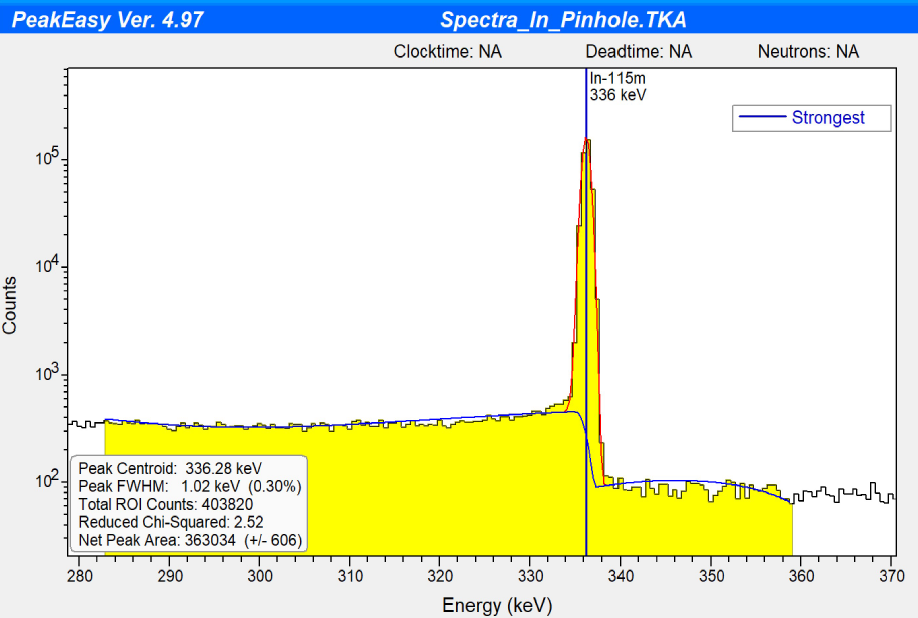
\includegraphics[width=\linewidth]{Figures/PeakEZ.png}
		\caption{336 keV In-115m peak counts determined using Peak Easy.}
		\label{fig:peakez}
	\end{figure}
% The background subtraction looks terrible.  It probably doesn't affect the answer, but this can be shown better.  Otherwise, it is an easy target for a reviewer.
	\ There was general agreement between the counts for In-115m and In-116m. 
The counts identified by LLNL resulted in 361,000 $+/-$ 0.23\% for In-115m and 1,383 $+/-$ 2.89\% for In-116m. 
The calculated results from Peak Easy determined 364,000 $+/-$ 0.38\% for In-115m and 1,402 $+/-$ 3.8\% for In-116m. 
It is expected that multiple peaks were used in the LLNL results thereby lowering the overall uncertainty.
A summary of the foils and reactions used for the snout experiment is given in Table \ref{Table:NIF}. The value of ``sig-phi'' was a STAYSL. calculated reaction rate used for the unfolding of the source spectrum.
	
	\begin{table}[]
		\caption{Activation information for the NIF experiment foils.}
		\label{Table:NIF}
		
		\centering
		\resizebox{\columnwidth}{!}{%
		\begin{tabular}{|c|c|c|c|c|c|c|}
			\hline
			\multicolumn{7}{|c|}{Kinematic Base} \\ \hline
			isotope & mass (g) & A0 (Bq) & N0 (nuclei) & \begin{tabular}[c]{@{}c@{}}Percent \\ Error\end{tabular} & \begin{tabular}[c]{@{}c@{}}Gamma\\  Self \\ Shielding\end{tabular} & \begin{tabular}[c]{@{}c@{}}"sig-phi"\\ (at/at-s)\end{tabular} \\ \hline
			Au196g & 3.733 & 5.74E+02 & 4.42E+08 & 1.60 & 0.974 & 3.98E-14 \\ \hline
			Au198 & 3.733 & 6.63E+02 & 2.23E+08 & 1.20 & 0.980 & 1.99E-14 \\ \hline
			In115m & 14.35 & 5.57E+03 & 1.30E+08 & 1.20 & 0.950 & 1.82E-15 \\ \hline
			In116m & 14.35 & 2.12E+05 & 9.97E+08 & 1.60 & 0.998 & 1.33E-14 \\ \hline
			Zr89 & 12.555 & 1.13E+03 & 4.61E+08 & 1.50 & 0.980 & 5.59E-15 \\ \hline
			Na-24 & 12.56 & 3.63E+03 & 2.83E+08 & 7.90 & 0.993 & 1.02E-15 \\ \hline
			\multicolumn{7}{|c|}{Basket} \\ \hline
			Au196g & 0.9393 & 9.47E+02 & 7.29E+08 & 1.20 & 0.974 & 2.61E-13 \\ \hline
			Au198 & 0.9393 & 2.00E+02 & 6.72E+07 & 1.20 & 0.980 & 2.39E-14 \\ \hline
			In115m & 0.4189 & 9.30E+02 & 2.17E+07 & 1.20 & 0.950 & 1.04E-14 \\ \hline
			In116m & 0.4189 & 1.69E+04 & 7.91E+07 & 2.80 & 0.998 & 3.61E-14 \\ \hline
			Zr89 & 0.2626 & 1.76E+02 & 7.15E+07 & 1.10 & 0.980 & 4.15E-14 \\ \hline
			Na-24 & 0.0962 & 4.11E+02 & 3.20E+07 & 1.20 & 0.993 & 1.50E-14 \\ \hline
			\multicolumn{7}{|c|}{Pinhole} \\ \hline
			Au196g & 0.148 & 6.97E+03 & 5.37E+09 & 1.30 & 0.974 & 1.22E-11 \\ \hline
			Au198 & 0.148 & 1.07E+02 & 3.58E+07 & 5.30 & 0.980 & 8.08E-14 \\ \hline
			In115m & 1.182 & 1.23E+05 & 2.87E+09 & 0.70 & 0.950 & 4.88E-13 \\ \hline
			In116m & 1.182 & 1.53E+05 & 7.18E+08 & 2.00 & 0.998 & 1.16E-13 \\ \hline
			Zr89 & 1.008 & 2.77E+04 & 1.13E+10 & 1.00 & 0.980 & 1.71E-12 \\ \hline
		\end{tabular}
	}
	\end{table}
	
	\subsection{Unfolding NIF Experiment with STAYSL}
	\ STAYSL has several modules that are used to unfold the neutron spectrum from the calculated activities. 
The main components used in this analysis are SHIELD, SIG-PHI Calculator, and PNNL STAYSL. 
The Beam Correction factor was not used because the NIF irradiation time is much less than the half-lives of the reaction products. 
	 
	\ A complete walk-through of the analysis is available on Github \cite{Me}. 
SHIELD was used to generate energy dependent neutron self-shielding factors for non-threshold reactions. 
SHIELD is not used on high energy threshold reactions because there is negligible shielding. 
	
	\ The SIG-PHI Calculator was used to consolidate all of the reaction information. Additionally, this module generates gamma-ray shielding factors. 
The input was generated from this information and the nuclei production information. % This sentence is unclear 
	
	\ STAYSL requires a starting guess spectrum. 
For this work, the NIF source was binned into the 140 group STAYSL structure, and the flux was scaled by the spherical divergence to the foil locations. 
	
	\ STAYSL was run for the pinhole, basket, and kinematic base for two cases. 
First, a guess spectrum  of the NIF source % which nif source?  Figure 5?
was used with 100 percent flux uncertainty up to 13 MeV. % Why? Not clear to the reader
The flux uncertainty from 13-15 MeV was set to five percent for the pinhole based on the reaction cross-section and threshold reactions expected results. % Not following
Less was known about the resultant spectra for the kinematic base and basket, so the 13-15 MeV flux uncertainty was set to 100 percent. 
STAYSL was ran iteratively using STAYSL.py %What is this; it was never introduced
until the $\chi^{2}$ changed by less than 0.1. 
The product spectrum is used as the guess spectrum for subsequent iterations. 
The flux uncertainty was not updated until the solution converged based on the $\chi^{2}$.
% If memory serves me, I found worse results when I did not update the uncertainty 
The degrees of freedom ($\nu$) for the pinhole is 4, because there are 5 foils. The other sets have 5 degrees of freedom.  % This sentence is randomly placed.
	
	The second method of iteratively solving started with a flat guess spectrum. 
A flat guess spectrum utilizes no a priori information about the flux, so it is a good indicator if the result matches up with the NIF guess spectrum iterations. 
The flat guess spectrum started with 100 percent uncertainty in all energy groups. 
	
	\section{Results}
% I didn't do a ton here since there are some unanswered questions and it seems the results may change.  As of now, these are highly suspect, so it would be interesting to see when using the guess spectrum from a simualtion.  That guess spectrum should be added to the plots.	
	
	\begin{figure}[t!]
		\includegraphics[width=\linewidth]{Figures/PinBothLog.png}
		\caption{Unfolded Spectrum for pinhole starting with NIF and flat guess.}
		\label{fig:pin}
		\vskip 0.9cm
		\includegraphics[width=\linewidth]{Figures/BaskBothLogZoomed.png}
		\caption{Unfolded Spectrum for the basket starting with NIF and flat guess (Truncated at 1 \text{$n-cm^{-2}$)}.}
		\label{fig:bask}
		\vskip 0.9cm
		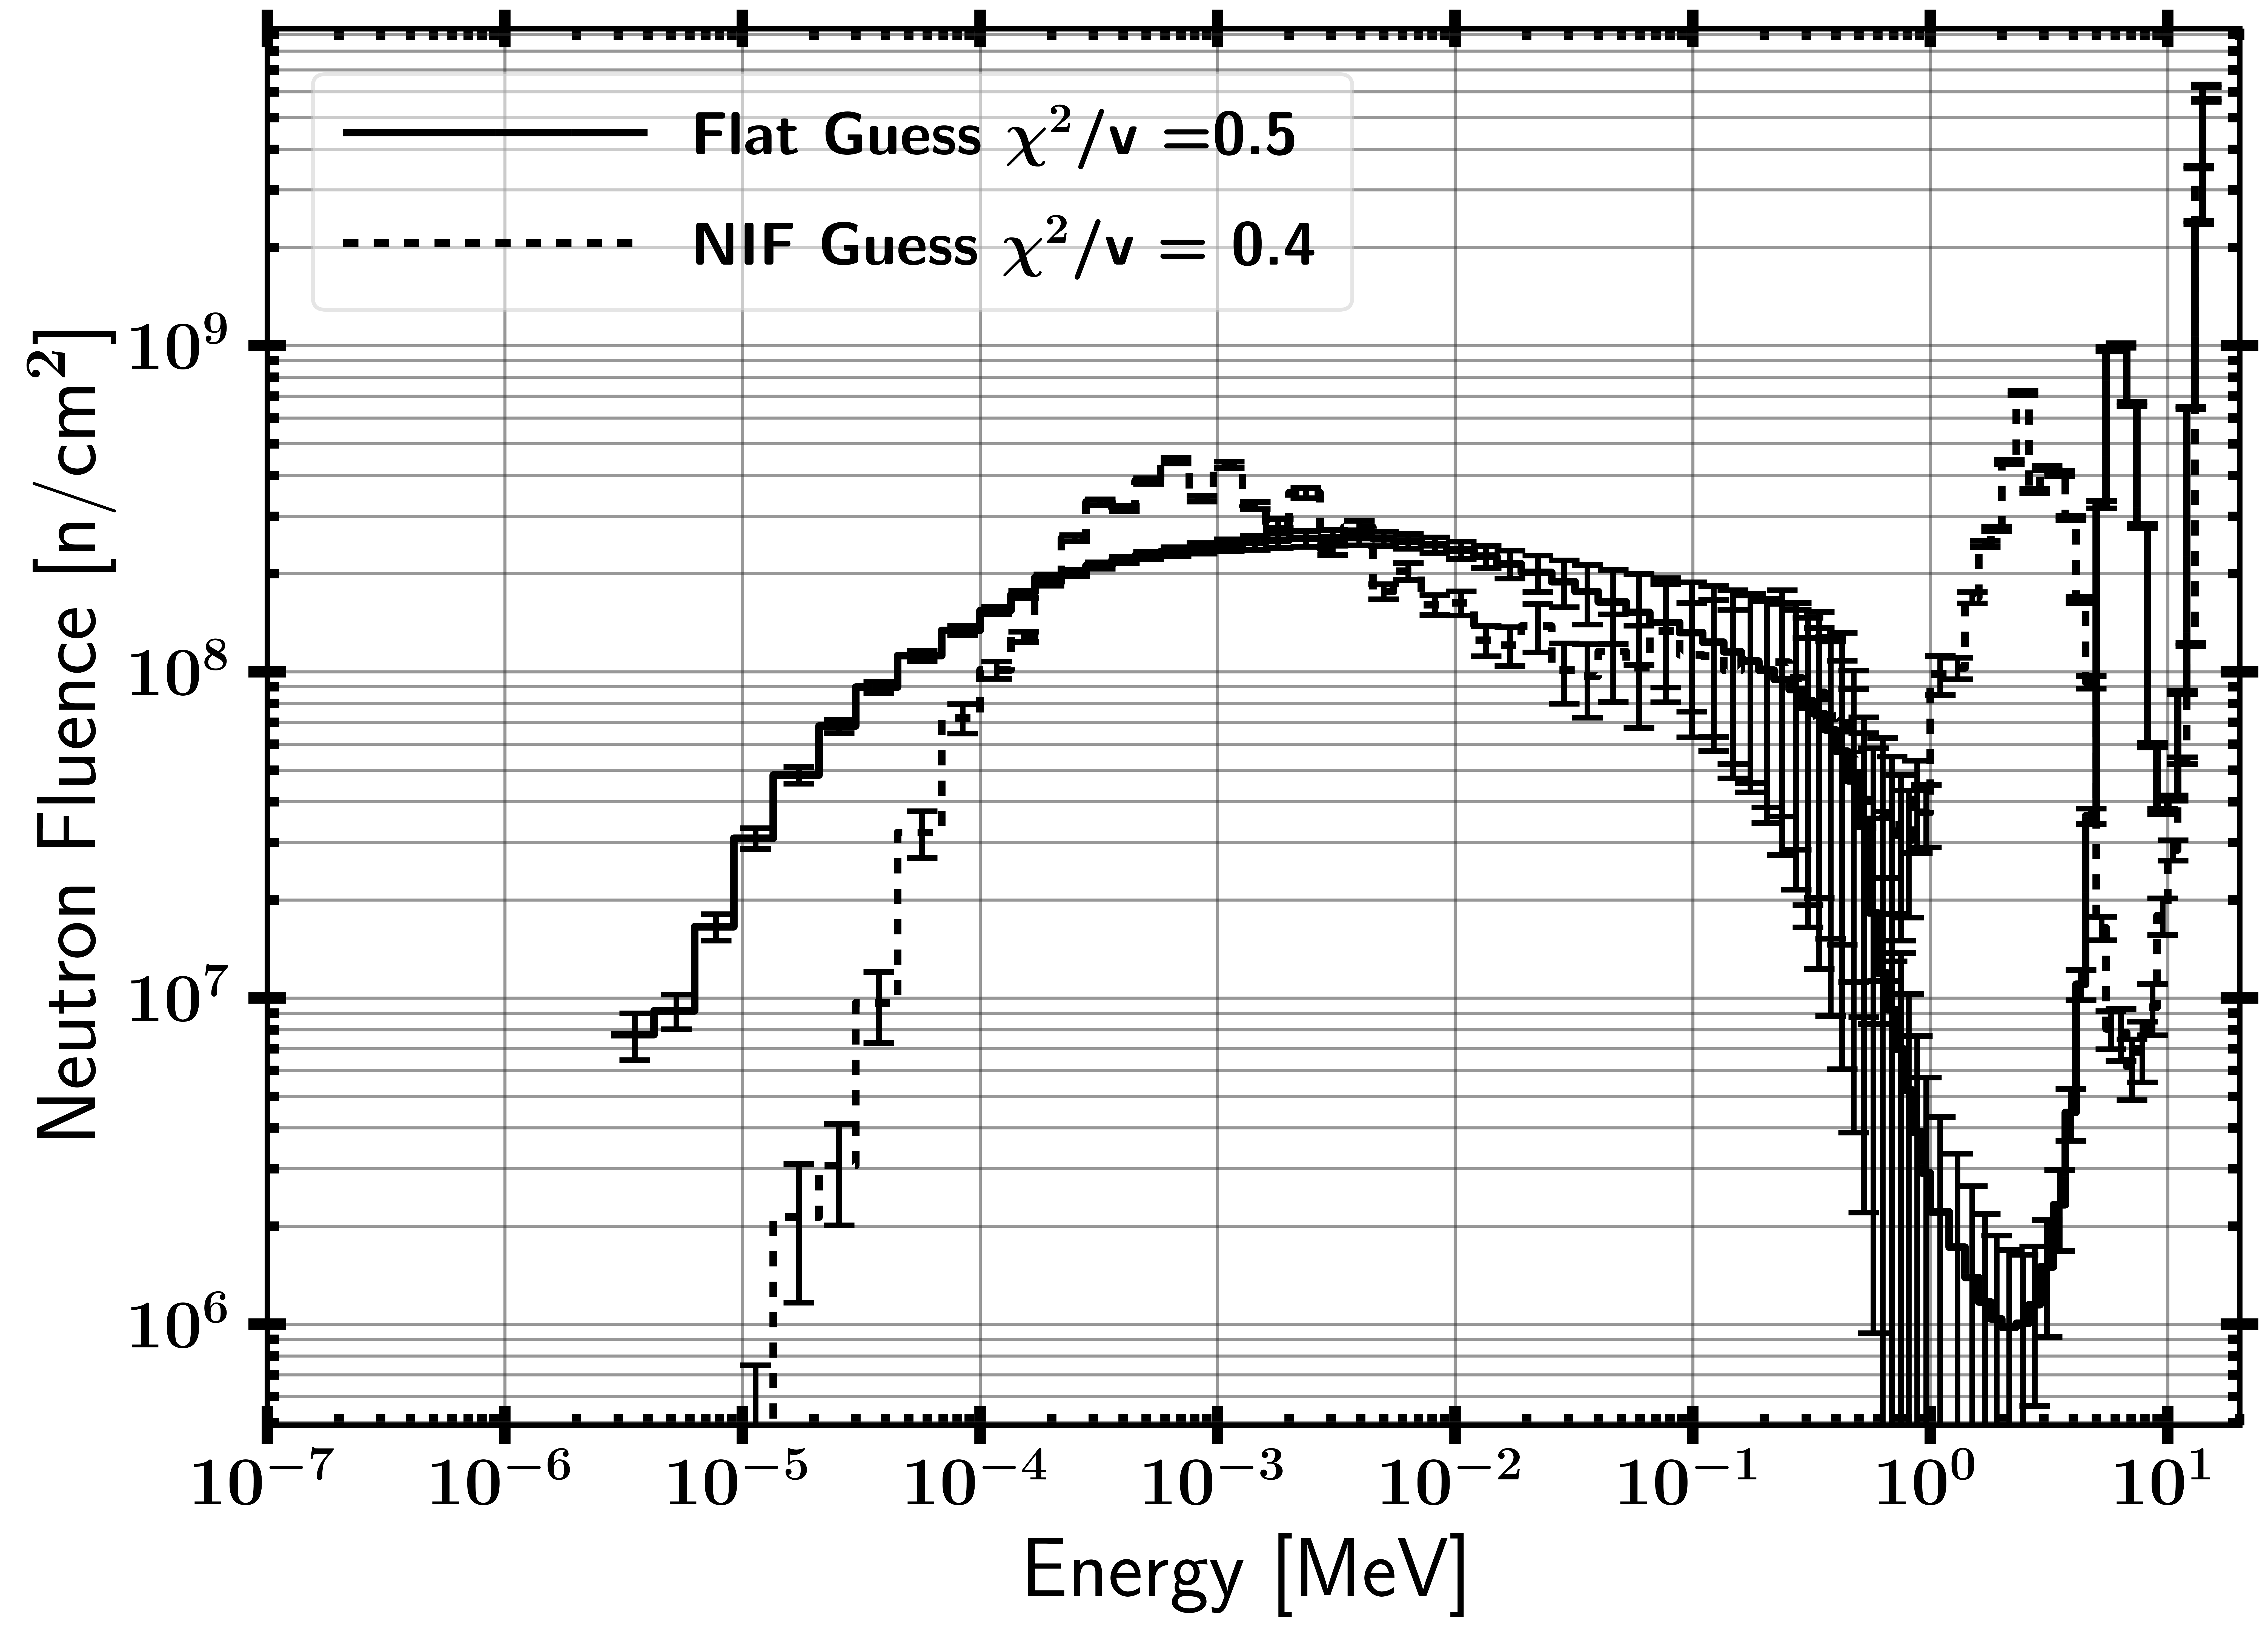
\includegraphics[width=\linewidth]{Figures/KBASBothLog.png}
		\caption{Unfolded Spectrum for the kinematic base starting with NIF and flat guess.}
		\label{fig:kbas}
		
	\end{figure}
	\ The unfolded results from STAYSL for the pinhole, basket, and kinematic base are shown in Figures \ref{fig:pin} - \ref{fig:kbas}. 
A summary of the $\chi^{2}$ values and associated p-values are provided in Table \ref{Table:STAY}. 
The basket results are truncated to a minimum fluence of 1 \text{$n-cm^{-2}$}. 
	
	\begin{table}[h]
		\caption{Summary of unfolded results for pinhole, basket, and kinematic base.}
		\label{Table:STAY}
		\centering
		\begin{tabular}{|c|c|c|c|}
			\hline
			Location & $\chi^{2}$ / $\nu$ & $\nu$ & p-value \\ \hline
			Pin NIF Guess & 4.4 & 4 & 0.0015 \\ \hline
			Pin Flat Guess & 6.6 & 4 & 3e-5 \\ \hline
			Basket NIF Guess & 18.7 & 5 & 1e-18 \\ \hline
			Basket Flat Guess & 17.7 & 5 & 1e-17 \\ \hline
			Kinematic Base NIF Guess & 0.35 & 5 & 0.88 \\ \hline
			Kinematic Base Flat Guess & 0.53 & 5 & 0.78 \\ \hline
		\end{tabular}
	\end{table}
	
	\ The results show good generally good agreement between the NIF guess and flat spectrum. 
No modeling information was available to use as a guess spectrum. % This should be used in the methods section where you were describing how you got the guess spectrum
The $\chi^{2}$ values can be iterated to shrink the value; however, care must be exercised in how many iterations to perform as non-physical results might be created. 
	
	\ The pinhole results in Figure \ref{fig:pin} show that there is a steep decrease in flux as energy decreases, which was not expected.  %Why not?  I think you mean the deep minimum was not expected.
The high energy bins at 13-15 MeV have very good agreement with expected values; however, the rest of the spectra was unexpected to some extent. 
The large epithermal peak energy is approximately 800 keV; which is approximately the first excited state in Al-27 (843 keV).
There is no physical basis for the near complete removal of neutrons between 1 and 10 MeV, while the source distribution indicates there should be a large portion present. 
The peak is shaped like an neutron evaporation spectrum. Past the epithermal peak, there is a decaying thermal tail. 
Starting from a flat spectrum produced nearly identical results, so it would have been ideal to have a threshold reaction near 1 MeV. 
The p-values for the pinhole indicate the result is very likely in both cases. % Is this true? P < 0.05 or P > 0.95 being the goal?  A quick explanation of a good P value and its meaning is needed.
Again, there is some degeneracy in the solution. 
	
	\ The basket results are similar to the pinhole with some key differences. 
First, the main 13-15 MeV peak has dropped by approximately six orders of magnitude, which is not representative of the linear attenuation of 34 cm of aluminum ($\Sigma$ $\approx$ 0.1 cm$^{-1}$). 
There is good agreement between the flat and NIF guess spectrum, so the threshold reactions are indicating the dropoff. 
Second, the neutron flux between approximately one to ten MeV is nearly removed. 
There is not a process that would remove all of the source neutrons in this region, but the result appears for the flat starting spectrum as well. 
The last difference is that the 800 keV peak only is present in the flat spectrum, and both guess spectra result in a peak at approximately 40 keV. 
The p-values for both spectra indicate that the result matches the activation. 
The result may have been improved with a better initial guess. 
	
	\ The kinematic base has the largest variance in results. 
At 13-15 MeV, the neutron flux is at approximatley $10^{9}$, which is more in line with expectations. 
The NIF guess and flat guess both have an epithermal energy peak; however, the location is different. 
In both spectra there is a large thermal tail from scattering. 
The results for the kinematic base are likely the farthest from the true distribution as the initial guess spectrum was farthest from reality. 
The p-values for the kinematic base indicate that the resultant spectra are not indicative of the neutron environment. 
	 
	\section{Conclusions}
	
	\ Characterizing the neutron energy spectrum in the snout experiment at the NIF provided mixed results. 
The foil activities and underlying nuclear data were applied in STAYSL to unfold the spectrum with STAYSL for the pinhole, basket, and kinematic base locations in the snout. 
The results in each case were not expected. 
An epithermal peak was produced and higher energy neutrons were removed, which does not align with anticipated results. 
The reduced $\chi^{2}$  result indicated that the pinhole and basket unfolds matched the activation results. 
	
	\ The unfolded neutron spectrum results highlight and reinforce necessity of having an initial guess spectrum for the generalized least-squares minimization. 
Each unfold, completed with the NIF starting spectrum and a flat spectrum, produced similar results; however, there are some differences that require attention. 
The kinematic base in particular did not converge to a similar solution over a large energy range. 
The results presented would be improved with a better starting guess for the initial spectrum. 

	\ifCLASSOPTIONcaptionsoff
	\newpage
	\fi
	
	\begin{thebibliography}{CLYC}
		% 1
		\bibitem{Knoll} 
		G. F. Knoll, Radiation Detection and Measurement, Ann Arbor,
		Michigan: Wiley, 2010.
		\bibitem{NETF}
		“AF NETF Graphite Standard Pile”, WADD-TR-61-174, Air Force Systems Command (1962).
		\bibitem{Will}
		W. Johnston, “Characterizing the Neutron Energy Distribution of the AFIT Building 470 Graphite Pile,” NENG 725, 2018.
		\bibitem{Bevins}
		J. E. Bevins, “Calibration of AFIT Graphite Pile to Account for 241Am Ingrowth in the 239PuBe13 Source,” Air Force Institute of Technology, Wright-Patterson Air Force Base, OH, 2009. 
		\bibitem{Bogetic}
		S. Bogetic, “Passive 18x Snout on TANDM 90-348,” University of California - Berkeley, 2018.  
		\bibitem{Luciano2012a}
		N. P. Luciano, “A High-Energy Neutron Flux Spectra Measurement Method for
		the Spallation Neutron Source,” Master's thesis, University of Tenessee Knoxville,
		2012.
		\bibitem{Kuijpers1977}
		L. Kuijpers, R. Herzing, P. Cloth, D. Filges, and R. Hecker, “On the Determination of Fast Neutron Spectra with Activation 
		Techniques; its Application in a Fusion Reactor Blanket Model,” Nuclear Instruments and Methods, vol. 144, no. 2, pp. 215-224, 1977. 
		\bibitem{Vagena2018b}
		E. Vagena, K. Theodorou, and S. Stoulos, “Thick-foils activation technique
		for neutron spectrum unfolding with the MINUIT routineComparison
		with GEANT4 simulations," Nuclear Instruments and Methods in Physics
		Research, Section A: Accelerators, Spectrometers, Detectors and Associated
		Equipment, vol. 887, no. January, pp. 64-69, 2018.
		\bibitem{Leo}
		W. R. Leo, Techniques for Nuclear and Particle Physics Experiments, New York: Springer-Verlag, 1994. 
		\bibitem{Reginatto2010}
		M. Reginatto, “Overview of spectral unfolding techniques and uncertainty esti-
		mation,” Radiation Measurements, vol. 45, no. 10, pp. 1323-1329, 2010.
		\bibitem{Perey1977}
		F. G. Perey, “Least-Squares Dosimetry Unfolding: The Program STAY'SL
		(ORNL/TM-6062),” Oak Ridge, Tennessee, 1977.
		\bibitem{Greenwood2016}
		L. Greenwood and C. Johnson, “Least-Squares Neutron Spectral Adjustment with
		STAYSL PNNL," EPJ Web of Conferences," vol. 106, p. 07001, 2016.
		\bibitem{Me}
		N. J. Quartemont, "NIF ETA," August 2018. [Online]. Available:
		https://github.com/nickquartemont/NENG612
	\end{thebibliography}
	
\end{document}


